\documentclass[12pt,a4paper, halfparskip]{scrartcl}
\usepackage[utf8]{inputenc}
\usepackage[ngerman]{babel}
\usepackage[T1]{fontenc}
\usepackage{amsmath}
\usepackage{amsfonts}
\usepackage{amssymb}
\usepackage{graphicx}
\usepackage[bookmarksnumbered,pdftitle={Name}]{hyperref}
\usepackage[left=2cm,right=2cm,top=2cm,bottom=2cm]{geometry}
\usepackage{lmodern}
\usepackage{listings}
\usepackage{xcolor}
\usepackage{tabularx}
\usepackage{booktabs}
\usepackage{pifont}
\usepackage{amssymb}
\usepackage{adjustbox}
\usepackage{cite}

\usepackage{geometry}
\geometry{a4paper, top=25mm, left=40mm, right=40mm, bottom=30mm,
headsep=10mm, footskip=12mm}

\title{Funktionsumfang und Leistungsfähigkeit kommerzieller und wissenschaftlicher NLP-Plattformen im Web}
\author{AUTOREN EINTRAGEN}
\renewcommand*{\titlepagestyle}{empty}

\definecolor{background}{HTML}{FFFFFF}

\lstdefinelanguage{json} {
    basicstyle=\normalfont\ttfamily,
    numbers=left,
    numberstyle=\scriptsize,
    stepnumber=1,
    numbersep=8pt,
    showstringspaces=false,
    breaklines=true,
    frame=lines,
    backgroundcolor=\color{background},
}

\begin{document}

\begin{titlepage}
	\centering
	
\includegraphics[width=1\textwidth]{Unilogo}\par\vspace{1cm}
	{\scshape\LARGE Universität Leipzig \par}
	\vspace{0.5cm}
	{\scshape\Large Abteilung Datenbanken \par}
	\vspace{0.2cm}
	{\scshape\large Big Data - Praktikum \par}
	\vspace{1cm}
	{\huge\bfseries Konzeptioneller Entwurf zum Thema \\ \textit{"Traffic Analysis with Deep Learning"} \par}
	\vspace{1cm}
	{\Large Ali Al-Ali und Jeremy Puchta \par}

	\vfill
	
	{\large \today\par}
\end{titlepage}

\newpage

\thispagestyle{empty}
\pagenumbering{Roman}
\tableofcontents
\addcontentsline{toc}{section}{Inhaltsverzeichnis}

\newpage
\pagestyle{empty}
\listoffigures
\addcontentsline{toc}{section}{Abbildungsverzeichnis}

\newpage
\listoftables
\addcontentsline{toc}{section}{Tabellenverzeichnis}

\newpage
\pagenumbering{arabic}
\newpage
\section{Einleitung}

Die vorliegende Ausarbeitung dokumentiert die Konzeption des Projekts \textit{Traffic Analysis with Deep Learning}.

Das Ziel des Projekts ist die Erstellung einer Webanwendung, welche Daten über das 
Verkehrsaufkommen am Leipziger Ring sammelt, statistisch analysiert und visualisiert.
Als Datengrundlage werden die unter \url{https://www.l.de/webcam.html} öffentlich bereitgestellten Webcambilder
des Leipziger Rings verwendet. 
Diese werden regelmäßig mithilfe eines Webscraping-Algorithmus abgerufen und dem Datensatz hinzugefügt (\textbf{T1}). 

Innerhalb der gesammelten Bilddateien werden die für das aktuelle Verkehrsaufkommen relevanten Objekte erfasst.
Dazu wird ein für den Anwendungsfall der Objekterkennung vortrainiertes neuronales Netz implementiert.
Der Leistungsstand des neuronalen Netzes wird im ersten Schritt untersucht, bevor im zweiten Schritt eine
Verbesserung der Leistungsfähigkeit vorgenommen wird (\textbf{T2}). 
Anschließend erfolgt die Transformation der gesammelten Bilddaten in Zeitreihendaten (\textbf{T3}). 

Abschließend wird der Zeitreihendatenbestand für die nachfolgende Analyse und Visualisierung innerhalb der 
Webanwendung aufbereitet. 
Die Webanwendung stellt ein Dashboard zur Verfügung, welches die aufbereiteten Verkehrsdaten grafisch 
visualisiert (\textbf{T4}). 

Die aufbereiteten Verkehrsdaten geben Informationen über die gegenwärtige Verkehrslage am Leipziger Ring preis 
und ermöglichen es Rückschlüsse auf mögliche Über- oder Unterlastungen des betrachteten Verkehrsbereich zu ziehen.
Aus diesen Analysen ist es möglich Handlungen für eine Verbesserung der Verkehrssituation abzuleiten.  
Daher sind die Ergebnisse der Ausarbeitung von Interesse für politische Amtsträger, Studenten verschiedener 
Fachrichtungen sowie interessierte Bürger der Stadt Leipzig.
\section{Technologiestack}

% Im Folgenden soll der Aufbau der Anwendung näher beleuchtet werden.
% Zunächst erfolgt die Präsentation des verwendeten Technologiestacks. 
% Anschließend werden die eingesetzten Komponenten vorgestellt und ein Überblick über ihre Funktionsweise geliefert.
% Für einen besseren Überblick über die Anwendung wird die Gesamtarchitektur mit Hilfe eines UML-Komponentendiagramms 
% visualisiert.

% \subsection{Architektur}

% Zur Erkennung von relevanten Objekten wird die \textit{YOLO}-Architektur genutzt.
% Bei \textit{YOLO} handelt es sich um ein Architekturmodell zur Objekterkennung.
% Die verwendete \textit{YOLO}-Implementierung heißt \textit{Darknet}. 

% % // Darkflow --> Implementiert Tensorflow

% Im Rahmen der Webanwendung wird eine Client-Server-Architektur eingesetzt. 
% Auf Serverseite wird das leichtgewichtige Framework \textit{Flask} genutzt.
% Im Frontend kommt die von \textit{Facebook} entwickelte JavaScript-Library \textit{React} zum Einsatz.
% Das Deployment erfolgt mit Hilfe der Containervirtualisierungs-Plattform \textit{Docker}.

% % des von \textit{Google} 
% % entwickelten Deep Learning - Frameworks \textit{Tensorflow} realisiert. 

% \subsection{Trainieren und Testen}

% Zur Verbesserung der Ergebnisse des vortrainierten Modells wird dieses mithilfe einer Vielzahl eigener Daten trainiert.
% Die Trainingsdaten werden zur ihrer Verwendung vorbereitet, das heißt dass die relevanten Objekte händisch 
% \textit{gelabelt} werden. Als relevante Objekte werden im Projektkontext PKWs, LKWs, Busse sowie Motorräder betrachtet.

% \subsection{Ablauf}

% Im ersten Schritt wird das aktuell öffentlich verfügbare Bild der Webcam \textit{gecrawled}. 
% Dieses wird als Input für das neuronale Netz eingesetzt und mit Hilfe des vortrainierten Modells analysiert.
% Als Ausgabe werden die auf dem Bild befindlichen, als relevant deklarierten, Objekte mit einem \textit{Confidence}-Wert
% zurückgegeben. 
% Der \textit{Confidence}-Wert stellt die Wahrscheinlichkeit dar, dass es sich um das jeweilige gekennzeichnete Objekt handelt.


\section{Architektur}

In diesem Kapitel erfolgt die Präsentation der Architektur der visionierten Webanwendung.
Das UML-Komponentendiagramm in Abbildung \ref{Architektur} visualisiert die Bestandteile der Anwendung.  

\begin{figure}[h!]
    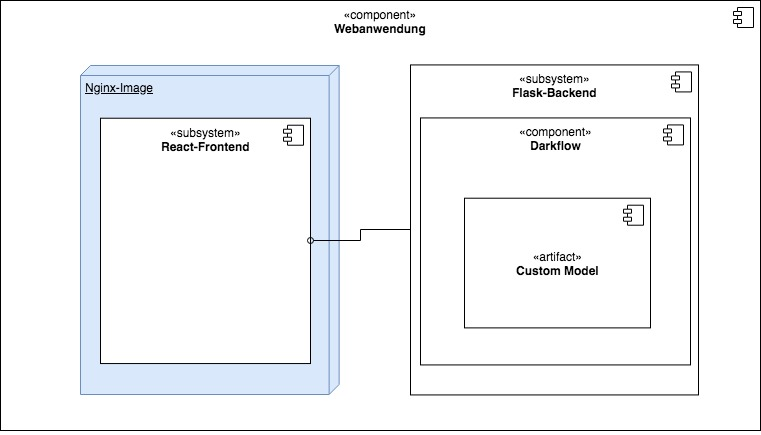
\includegraphics[width=\linewidth]{resources/images/bigdata-prak-arch_recent.jpg}
    \caption{Architektur der visionierten Webanwendung}
    \label{Architektur}
\end{figure}

Zur Identifizierung von relevanten Objekten wird die \textit{YOLO}-Architektur genutzt.
Bei \textit{YOLO} handelt es sich um ein neuronales Netz, dass zum detektieren sowie zum lokalisieren von Objekten entworfen wurde.
Die in diesem Projekt verwendete \textit{YOLO}-Implementierung heißt \textit{Darkflow}. 

Die Webanwendung basiert auf einer Client-Server-Architektur.
Auf Serverseite wird das leichtgewichtige Python-Framework \textit{Flask} genutzt.
Flask wurde mit dem Ziel entwickelt seinen Nutzern einen einfachen und schnellen Einstieg zu ermöglichen, 
jedoch mit der Möglichkeit bis hin zu komplexen Anwendungen zu skalieren (vgl. siehe \cite{palletsprojects}). 

Im Frontend kommt die von \textit{Facebook} entwickelte JavaScript-Library \textit{React} zum Einsatz.
Wie andere komponentenbasierte Frontend-Frameworks stellt auch \textit{React} einen komfortablen und schnellen 
Weg zur Erstellung von UI-Komponenten bereit (vgl. siehe \cite{react.js}). 
Die im Frontend erstellten Grafiken werden mithilfe von \textit{p5.js} erstellt.
Dabei handelt es sich wiederum um eine JavaScript-Library für die Erstellung von grafischen und interaktiven
Inhalten (vgl. siehe \cite{p5.js}). 

Sämtliche Komponenten des Systems werden mithilfe der Container\-virtualisierungs-Technologie Docker deployed.
Docker ermöglicht die Bereitstellung und den Betrieb von Linux-Containern.
Innerhalb dieser Container können Images deployed werden, die unter anderem auf \textit{Dockerhub} (\url{https://hub.docker.com/}) 
bereitgestellt werden (vgl. siehe \cite{redhat-docker}).
Im Rahmen des Projekts wird beispielsweise das offizielle Image des \textit{Nginx}-Webservers verwendet, um den 
Production-Build des Frontends bereitzustellen.



% Im Folgenden soll der Aufbau der Anwendung näher beleuchtet werden.
% Zunächst erfolgt die Präsentation des verwendeten Technologiestacks. 
% Anschließend werden die eingesetzten Komponenten vorgestellt und ein Überblick über ihre Funktionsweise geliefert.
% Für einen besseren Überblick über die Anwendung wird die Gesamtarchitektur mit Hilfe eines UML-Komponentendiagramms 
% visualisiert.

% \subsection{Architektur}

% Zur Erkennung von relevanten Objekten wird die \textit{YOLO}-Architektur genutzt.
% Bei \textit{YOLO} handelt es sich um ein Architekturmodell zur Objekterkennung.
% Die verwendete \textit{YOLO}-Implementierung heißt \textit{Darknet}. 

% % // Darkflow --> Implementiert Tensorflow

% Im Rahmen der Webanwendung wird eine Client-Server-Architektur eingesetzt. 
% Auf Serverseite wird das leichtgewichtige Framework \textit{Flask} genutzt.
% Im Frontend kommt die von \textit{Facebook} entwickelte JavaScript-Library \textit{React} zum Einsatz.
% Das Deployment erfolgt mit Hilfe der Containervirtualisierungs-Plattform \textit{Docker}.

% % des von \textit{Google} 
% % entwickelten Deep Learning - Frameworks \textit{Tensorflow} realisiert. 

% \subsection{Trainieren und Testen}

% Zur Verbesserung der Ergebnisse des vortrainierten Modells wird dieses mithilfe einer Vielzahl eigener Daten trainiert.
% Die Trainingsdaten werden zur ihrer Verwendung vorbereitet, das heißt dass die relevanten Objekte händisch 
% \textit{gelabelt} werden. Als relevante Objekte werden im Projektkontext PKWs, LKWs, Busse sowie Motorräder betrachtet.

% \subsection{Ablauf}

% Im ersten Schritt wird das aktuell öffentlich verfügbare Bild der Webcam \textit{gecrawled}. 
% Dieses wird als Input für das neuronale Netz eingesetzt und mit Hilfe des vortrainierten Modells analysiert.
% Als Ausgabe werden die auf dem Bild befindlichen, als relevant deklarierten, Objekte mit einem \textit{Confidence}-Wert
% zurückgegeben. 
% Der \textit{Confidence}-Wert stellt die Wahrscheinlichkeit dar, dass es sich um das jeweilige gekennzeichnete Objekt handelt.


\section{Ablauf}

Dieses Kapitel richtet den Blick auf den Ablauf des Systems. 
Dabei ist der Ablauf unterteilt in zwei unabhängige Phasen:

\begin{enumerate}
    \item Trainings- und Testingphase des neuronalen Netzes
    \item Betriebsphase der Webanwendung
\end{enumerate}

Zunächst wird der Ablauf der ersten Phase vorgestellt.
Diese befasst sich mit dem Training und Testing des neuronalen Netzes. 
Das verwendete neuronale Netz basiert auf der YOLO-Architektur, welche in [QUELLE] dokumentiert ist.
Weiterhin wird ein vortrainiertes Model zur Objekterkennung verwendet.
Dieses bietet bereits die Möglichkeit 80 Klassen zu erkennen und zu klassifizieren. 
Aufbauend auf diesem Fundament, wird das Model entsprechend der im Rahmen des Projekts aversierten Domäne optimiert.
Dabei spricht man von \textit{Training}.

Im Rahmen der Trainingsphase wird der zusammengestellte und mit Labeln versehene Datensatz verwendet, um 
das neuronale Netz zu trainieren. 
Hierbei werden die Bilder iterativ durch das neuronale Netz via \textit{Forward Pass}-Prozess [REFERENZ] geschickt.
Dabei detektiert und klassifiziert das neuronale Netz die im Bild vorliegenend Objekte und vergleicht anschließend
die Resultate mit den im Input-Datensatz manuell gelabelten Objekten.
Im Fehlerfall passt das neuronale Netz die Kantengewichte mit Hilfe der \textit{Back Propagation}-Technik [REFERENZ] an.
Zur Validierung des neuronalen Netzes werden dem Netz unbekannte Bilder als Input bereitgestellt.
Damit wird überprüft, ob das Netz in der Lage ist auf unbekannte Input-Daten zu reagieren und ob beispielsweise eine 
Überanpassung existiert.

Das Ergebnis der Trainingsphase ist ein auf den Projektanwendungsfall spezialisiertes Model.
Dieses Model wird im Folgenden in das Backend der Webanwendung integriert.
Zur Laufzeit der Webanwendung wird stündlich das aktuell veröffentlichte Webcambild (siehe \url{https://www.l.de/webcam.html}) gecrawled.
Dieses wird vom Flask-Backend durch das neuronale Netz geschickt. 
Das Resulat stellt die enthaltenen Objekte in einer JSON-Datei dar. 
Die enthaltenen relevanten Werte werden aus der JSON-Datei extrahiert und in eine Datenbank gespeichert.
Der gesammelte Datenbestand wird im Anschluss aufbereitet, harmonisiert und analysiert, bevor sie an das Frontend
geschickt werden.
Im Frontend werden die aus den Daten resultierenden Statistiken nutzerfreundlich visualisiert.


\newpage
\pagenumbering{arabic}

% Literaturverzeichnis
\newpage
\pagenumbering{Roman}
\setcounter{page}{4}
\pagestyle{empty}
\bibliographystyle{unsrt}
\addcontentsline{toc}{section}{Literaturverzeichnis}
\renewcommand{\refname}{Literaturverzeichnis} 
\bibliography{sources}

% ABKÜRZUNGSVERZEICHNIS
\newpage
\pagestyle{empty}
\section*{Abkürzungsverzeichnis}
\addcontentsline{toc}{section}{Abkürzungsverzeichnis}
<falls viele Abkürzungen vorkommen>
\begin{description}
	\item [TLA] Three Letter Acronym
\end{description}

% GLOSSAR
\newpage
\pagestyle{empty}
\section*{Glossar}
\addcontentsline{toc}{section}{Glossar}
\begin{description}
	\item[Angreifer] "`Eine Person, die eine ihm bekannte Verwundbarkeit ausnutzt, um ein Computersystem anzugreifen"'. 
\end{description}

% \end{footnotesize}

\end{document}